\def \Subject {تمرین امتیازی GSM}
\def \Course { امنیت سیستم های کامپیوتری}
\def \Author {ستاره باباجانی - ملیکا محمدی فخار}
\def \StudentNumber {99521109-99522086}

\begin{center}
\vspace{.4cm}
{\bf {\huge \Subject}}\\
\vspace{.3cm}
{\bf \Large \Course}\\
\vspace{.2cm}
{\bf \Author }  \\
{\bf شماره دانشجویی:\ \StudentNumber}\\
\end{center}

\hspace{\fill} 



\clearpage

%\huge{\Subject}\\[1.5 cm]
%\chapterauthor{\Author~ : \StudentNumber}
\begin{figure}[h!]
    \centering
    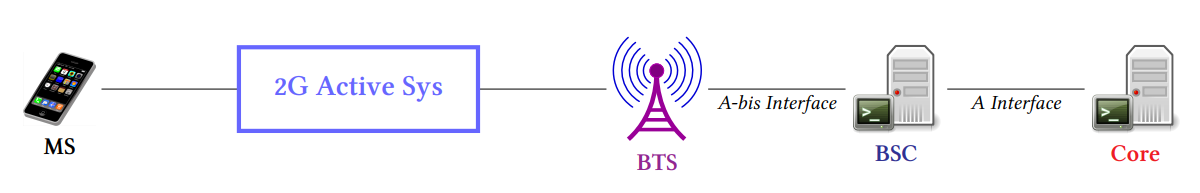
\includegraphics[width=0.9\linewidth]{images/1.png}
    \caption{نمای کلی}
    \label{fig:GSM}
\end{figure}


شبکه‌های GSM  Communications) Mobile for System (Global    از نوع شبکه‌های نسل دوم هستند که در اواخر دهه ۱۹۸۰ توسعه یافتند. این شبکه‌ها با مشکلات امنیتی زیادی از جمله قابلیت شنود ارتباطات توسط افراد خلافکار مواجه بوده‌اند. یکی از اصلی‌ترین مشکلات امنیتی در GSM ارتباطات Active Sys (System) است که می‌تواند باعث شنود و تخریب ارتباطات شود.
ارتباطات GSM در Active Sys به این شکل انجام می‌شود:



\section{مستر سیستم System) :(Master }
این سیستم یک دستگاه با قابلیت ارتباط با تلفن‌های همراه است که مسئول برقراری ارتباط با تلفن‌های همراه و نیز متصل شدن به BTS ها می‌باشد.

\section{BTS Station) Transceiver :(Base   }
BTS ها مسئول ارتباط با تلفن‌های همراه در یک منطقه خاص هستند.
تلفن‌های همراه از طریق BTS ها با مستر سیستم متصل می‌شوند.
همچنین از جمله تجهیزات مورد استفاده توسط Sys Active GSM دستگاه‌هایی با نام Catcher IMSI می‌باشند که قادر به شنود ارتباطات تلفن‌های همراه و همچنین نفوذ به وسط ارتباطات بین دستگاه و شبکه می‌باشند.



\section{عملکرد Sys Active :GSM}
مستر سیستم به صورت غیرقانونی یک BTS نادرست ایجاد می‌کند که با تلفن‌های همراه ارتباط برقرار می‌کند. تلفن‌های همراه به عنوان بالماسک تلقی می‌شوند و به این BTS متصل می‌شوند.
بعداً این مستر سیستم می‌تواند ارتباط بین تلفن‌های همراه و BTS را برقرار کرده و همچنین از طریق تلفن‌های همراه عملیات شنود را انجام دهد.
Project) Partnership Generation 3rd (The 3GPPبه عنوان یک سازمان استانداردهای تلفن همراه، تلاش‌های زیادی برای بهبود امنیت شبکه‌های GSM انجام داده است. این تلاش‌ها به صورت مستمر انجام می‌شوند و به مرور زمان امنیت شبکه‌های GSM بهبود یافته است.
باید توجه داشت که استفاده از IMSI Catcher و نفوذ به ارتباطات GSM به شدت غیرقانونی است و با قوانین حریم خصوصی و امنیت مخابراتی در تضاد است. افرادی که از این نوع تجهیزات برای انجام فعالیت‌های غیرقانونی استفاده می‌کنند ممکن است مورد پیگرد قانونی قرار گیرند. امنیت اطلاعات و ارتباطات تلفن همراه اهمیت زیادی دارد و باید توسط مراجع مختصرین تعدیل و پیگیری شود.
